\newsavebox{\Mechanismgraphicbox}
\begingroup
\makeatletter
\let\Mechanismoriginalendfloatbox\@endfloatbox
\def\@endfloatbox{\Mechanismoriginalendfloatbox
\typeout{MECH-FLOAT-HEIGHT=\the\ht\@currbox}
\typeout{MECH-FLOAT-DEPTH=\the\dp\@currbox}}
\makeatother
\begin{figure*}[t]
  \centering
  \sbox{\Mechanismgraphicbox}{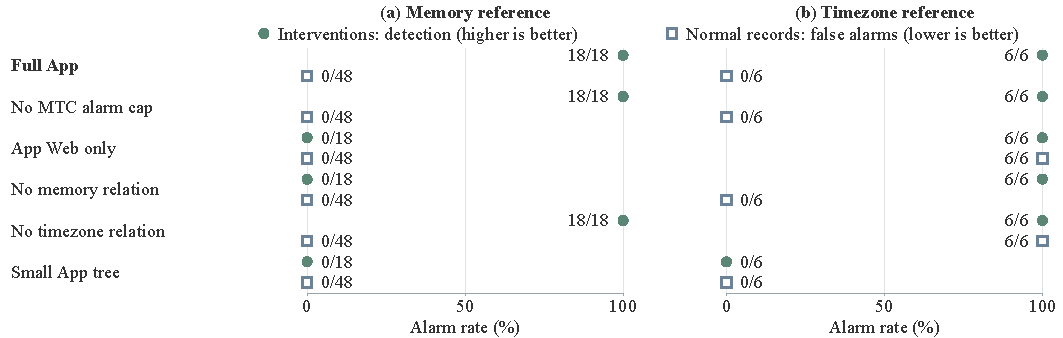
\includegraphics[width=\textwidth]{figures/F03a_F04_main.pdf}}
\typeout{MECH-TEXTWIDTH=\the\textwidth}
\typeout{MECH-TEXTHEIGHT=\the\textheight}
\typeout{MECH-GRAPHIC-WIDTH=\the\wd\Mechanismgraphicbox}
\typeout{MECH-GRAPHIC-HEIGHT=\the\ht\Mechanismgraphicbox}
\typeout{MECH-GRAPHIC-DEPTH=\the\dp\Mechanismgraphicbox}
\usebox{\Mechanismgraphicbox}
  \caption{Saved Native-App Web reference evaluations for memory (a) and timezone (b). Positions show alarm rates; labels show T/N. Intervention alarms indicate detection (higher preferred); normal alarms indicate false alarms (lower preferred). Memory: 18 effective interventions, 48 normal controls; six separate no-change operations yield 0/6 alarms for every method. Timezone: six App Web interventions and six normal system changes; the latter belong to 30 normal records. Counts hold separately for all three frozen configurations. Equal aggregates are displayed without pooling denominators. These development materials are not a new blind test. Broader normal-record costs are reported separately; specialist zeros do not establish generally low false alarms.}
  \Description{Six shared method rows compare saved complete App methods in two aligned panels. Each row has a filled green intervention-detection circle and a hollow blue normal-false-alarm square. Positions encode alarm rates on the same zero-to-one-hundred-percent scale, with exact T/N counts. Symbols are offset vertically, never horizontally. Memory uses eighteen interventions and forty-eight normal controls; timezone uses six App Web changes and six normal system changes. Counts hold separately for three frozen configurations.}
  \label{fig:app-reference-mechanisms}\label{fig:hybridguard-overview}
\end{figure*}
\endgroup
